\chapter{基于SVR+Q+MCKP分块模型在多渠道广告投放预算分配中的研究}

% 首先介绍多渠道广告投放资金分配问题使用强化学习研究的现状(没有利用强化学习解决该问题的文献,存在的主要问题:数据量较少,导致值函数估计不准确等问题,收敛速度慢,说明本文采用非参数化建模的原因,非参数化建模又存在什么问题,针对此问题又是如何解决的)
% 介绍深度强化学习
% 介绍本文提出的混合网络模型算法
% “我知道我的广告费有一半浪费了,可是我不知道浪费的是哪一半。”美国费城商人约翰·华纳梅克的这句自嘲式的调侃简直让人抓狂——似乎你绞尽脑汁想出的营销点子就是为了达到一个目的——尽量让广告费被浪费得少一点而已。

\section{直复营销下广告预算分配问题阐述}
本章,首先介绍了在直复营销体系下,基于第三方广告代理商进行广告投放的应用场景及其具体的投放过程。然后,说明了广告投放的目标是追求全渠道的基于ROI的LTV最大化,以此作为选择强化学习解决该问题的依据。最后,介绍了广告投放预算分配场景所具有的三个特点,并针对这些特点来针对性的提出解决方法,以优化强化学习算法,将此作为本章研究的出发点。

\subsection{广告预算分配场景}
美国直复营销协会(American Direct Marketing Association,ADMA)\footnote{http://www.the-dma.org/}将直复营销(Direct Response Marketing)定义为一种市场营销体系,运用一种或几种广告媒介在任何地点产生可以度量的反应或交易。直效营销仅仅属于直复营销中的一种应用场景,它特指不通过第三方,中间人,而直接对客户进行推广和营销,以维持企业与客户的良好关系。但是,在这种场景下需要企业有充足的客户资源和大量的相关客户资料,这对于大部分企业是很难办到的,需要很长时间的积累,特别是在日益激烈的市场竞争环境中,时间就是企业的生命线。于是,为了快速获取用户、推广相关产品、扩大公司的收入,越来越多的企业选择通过第三方广告代理商(Ad-agency)进行广告投放。

广告代理商除了帮助企业进行广告设计与策划以外,还有一部分更重要的工作,就是帮助广告主安排或代为购买媒介空间或时间。近年来,随着广告市场的不断发展和扩大,为了方便广告主高效的进行广告投放,大部分在线的广告代理商也都建设了自己的广告投放平台,其投放流程如图$\ref{fig:ad_process}$所示。在广告投放平台上,广告代理商(Ad-agency)有很多可供选择的广告渠道(channel)资源,广告主每次需要提供一个广告投放策略,策略的内容包括在哪些渠道上投放广告以及对应投放多少金额的广告费。然后,广告代理商会按照广告主提供的投放策略,将对应的广告量通过各渠道投放给潜在顾客(广告的受众)。在广告投放结束后,广告代理商会将此次广告投放的直观效果反馈给广告主,同时广告主也可以通过追踪已经交易的顾客的后续信息,综合评价此次的投放效果。

\begin{figure}[htbp]
\centering
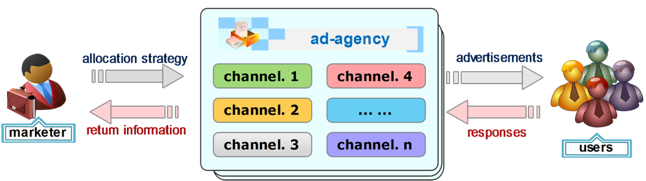
\includegraphics[width=0.8\textwidth]{ad_process}
\caption{基于ad-agence的广告投放过程}
\label{fig:ad_process}
\end{figure}

通过以上的介绍,可以看到在通过广告代理商投放广告的过程中,顾客可以及时接收到广告主发布的广告信息,而广告主也会收到响应顾客的响应反馈,因此广告主与顾客之间是存在互动性的。另外,广告主还可以根据广告代理商反馈的投放效果信息以及追踪用户未来行为等方式去量化此次广告投放对企业的价值,因此效果是可衡量性的,所以,利用广告代理进行广告投放的方式也属于直复营销体系。

在企业进行广告投放的真实业务中,为了保证财务帐面的稳定以及公司合理健康的发展,公司财务每个月都会给出该月的广告投放资金的预算,然后广告投放部门会在此预算下进行广告预算的合理分配,以使得公司的业务不断扩大、收入持续增长。但是,因为广告投放场景比较复杂,单纯靠广告投放人员制定预算分配策略往往很持续难达到好的效果,所以需要充分利用机器学习技术。

\subsection{基于渠道的LTV值}
通常情况下,企业在进行广告投放时,为了能够更好的评价广告渠道的质量,而且为了能达到持久有效的营销效果,一般都会选择一个广告代理商进行为期一年或几年的持续投放。因此,广告投放是一个序列化的过程。

评价广告投放渠道质量的重要指标是投资回报比(Return On Investment, ROI)即一定周期内,广告主通过广告投
放收回的价值占广告投入的百分比,计算方法如式\eqref{seq:roi}所示,其中Income表示收入额,Cost表示成本额,Investment表示投资额,一般情况下认为Cost和Investment是同一概念。
\begin{equation}\label{seq:roi}
\begin{aligned}
 ROI=\frac{Income-Cost}{Investment}*100\%
\end{aligned}
\end{equation}

然而,在广告投放的过程中,用户的反馈存在一定的延迟,而且某一时刻投放的广告会对后面时刻的广告投放效果产生一定程度的影响,所以不能仅仅使用即时的ROI值作为渠道质量的评价指标。比如,一个顾客在某一时刻看到某广告,但是并没有立刻产生正向反馈或者交易,而是在经过若干时间后的某一时刻才有正向反馈。那么,此时所产生的收益不单单与现在这个时刻的广告投放效果有关,还与之前的广告投放效果有关。所以,在计算广告投放所产生的回报时,应该要有全局观念。因此,在实际应用中,广告主一般将基于渠道LTV的ROI值作为选择广告渠道的指标,LTV是指渠道所产生的累积收益,只要将公式\eqref{seq:roi}中的Income换成渠道的LTV值即可。

考虑到企业进行广告投放的主要目的是为了尽可能的增加自身利润,如果单单只考虑渠道的ROI值,并不能得到对企业来说价值最大的投放策略。因为即使一个投放产生的ROI值很大,但是如果产生这个很大ROI值的那个投放花费很小的话,其利润不可能很大,这是不是企业所期望得到的最终效果。所以本章研究的给定预算下的广告投放资金分配问题,并不以ROI值作为评价指标,而是关注什么样的投放策略可以使企业产生的收益最大化,即广告渠道的LTV值最大。

通过第二章的介绍,我们知道,强化学习在处理序列问题时,因为考虑到了延迟奖赏的问题,并且以追求累积奖赏最大化作为优化目标,所以将强化学习技术应用在广告投放领域,可以充分发挥其优势,预期取得较好的结果。

\subsection{广告预算分配特点}
% 多渠道/总预算限制/数据量少
解决好广告投放的资金预算分配问题,虽然有着很高的现实意义和商业价值,但是目前并没有引起很多学者和专家的注意。其中,最主要的原因就是没有在此领域公开的数据集。本文的数据是基于国内某公司在进行广告投放过程中所产生的真实数据,所以研究内容具有的实用性和真实性。

即便拥有了相关的广告投放数据,但是因为该领域还存在诸如场景复杂、数据量较少、固定预算约束等问题,不能直接将强化学习算法应用在该场景中。所以,本章从这些存在的问题作为出发点,结合强化学习进行分析,并提出了相应的解决方法。

对于大部分企业来说,广告投放是以天为单位进行的,所以投放数据量比较少,影响了模型的训练和学习,因此,为了提高数据的使用率,在强化学习模型中我们考虑使用非参数化函数逼近的方法进行Q值函数的学习。另外,通常情况下,为了达到全方位的效果,在进行广告投放时会选择多个渠道同时进行投放,因此,我们不能只考虑渠道自身延迟反馈的影响,而且还应该考虑渠道间的相互影响。最后,每一次制定广告投放策略之前,都需要在给定的固定预算约束进行,所以,我们在使用强化学习进行Q值估计之后,还要考虑如何进行合理的分配预算资金。

\section{SVR-RBF+Q分块逼近模型}
在真实的广告投放场景中,广告主进行广告投放的周期是相对较长的(一天一次),所能得到的数据也就相对较少。所以,在进行Q值函数逼近值时,要求我们高效的利用仅有的训练样本。然而,通过第二章的介绍,我们知道在参数化函数逼近方法中,线性逼近值函数的逼近能力较弱、效率较低,非线性函数(神经网络)逼近又需要有充足的训练样本。所以,综合考虑,我们选择了基于非参数化函数逼近的模型,因为该模型是一种基于样本的学习方法,具有较高的灵活性,而且适用于小样本数据。

但是,非参数化函数逼近常常面临着收敛性难移保证的问题。于是,本章提出了基于SVR-RBF+Q的强化学习模型,在该模型中,将对Q值函数逼近问题转化为高维特征空间中的线性回归问题,从而可以加快函数的收敛速度。另外,为了在小数据集下提高函数逼近的精度,提出分块逼近的思想,每个离散的行为作为一块,分别使用SVR-RBF+Q模型进行训练,最后再利用训练好的分块模型多路逼近Q值函数。

\subsection{分块多路逼近思想}
经过前面的分析,我们知道,在广告投放场景中,可获得的数据量比较少,如果将所有渠道合在一起进行建模,很难拟合出可靠的值函数变化规律。所以,我们采取分渠道进行建模的思路。进一步地,每个渠道在进行值函数的逼近时,考虑到状态空间和行为空间(广告花费)是连续的,因为数据样本较少也会造成状态行为值函数逼近的不准确。

针对以上问题,本章提出分块多路逼近的思想。在离线学习时,首先,使用一种花费空间离散化的方法(下文会详细介绍),将花费空间离散成$K$个行为$A=\{a_{1},a_{2},\cdots,a_{K}\}$。然后,将原始训练样本<$\mathbf{s_{t}},c_{t},r_{t+1},\mathbf{s_{t+1}}$>中的花费$c_{t}$转换成相对应的离散行为$a_{t}$,并且按照样本中行为的类别将原始样本集划分为$K$个临时样本单元(即$K$个块),所以,每一个离散行为$a_{k}$对应一个临时样本单元$D_{k}^{'}=\{<\mathbf{s_{t}},a_{t},r_{t+1},\mathbf{s_{t+1}}>|t=1,2,\cdots,N_{k}\}$,$N_{k}$为该临时样本单元$D_{k}^{'}$中的样本个数,$\mathbf{s_{t}}$为当前状态向量,$\mathbf{s_{t+1}}$为后继状态向量。接着,针对每一个临时样本单元$D_{k}^{'}$,利用Q值函数的更新公式(算法$\ref{algo:algorithm_2}$中第7行)计算$Q(\mathbf{s_{t}})$值,形成带Q值的样本单元$D_{k}=\{<\mathbf{s_{t}},a_{t},r_{t+1},Q(\mathbf{s_{t}}),\mathbf{s_{t+1}}>|t=1,2,\cdots,N_{k}\}$。下一步,利用非参数化函数逼近模型Q对样本单元中的数据进行建模,Q$=\{\text{Q}_{k}|k=1,2,\cdots,K\}$,每个样本单元$D_{k}$对应一个只关于状态 $\mathbf{s}$的子模型$\text{Q}_{k}(\mathbf{s})$,且各个子模型之间是相互独立。最后,将分块后的$K$个子模型多路逼近Q值函数。在每一次迭代过程中,对每个样本单元中的样本按照Q值更新公式重新计算Q$_{k}(\mathbf{s})$,直到满足设定的停止条件。

\subsection{RBF-SVR+Q模型}
现介绍利用RBF-SVR+Q模型对第$k$个样本单元$D_{k}$进行Q$_{k}$值函数逼近的方法,对其他样本单元的建模过程与之相同。

为了简单起见,对样本单元$D_{k}$进行简化处理,只考虑当前状态向量和对应的$Q$值,即$\{(\mathbf{s_{i}}, Q_{i})\}_{i=1}^{N_{k}}\subseteq(\mathbf{X} \times \mathbf{Y})^{N_{k}}$,其中$\mathbf{s_{i}}$为样本的输入向量,$Q_{i}$为样本对应的Q输出值,$N_{k}$为第$k$个样本单元的数量,$\mathbf{X}$表示输入域,$\mathbf{Y}$表示输出域。我们的目标是使用基于核函数的支持向量回归(Support Vector Regression, SVR)的模型(RBF-SVR+Q)来拟合$\mathbf{s_{i}}$和$Q_{i}$之间的回归关系,即逼近Q值函数。

对样本单元$D_{k}$利用RBF-SVR+Q进行进行模型时,以结构化风险最小为目标,学习一个仿射函数$f:\mathbf{X} \mapsto \mathbf{Y}$。形式为:
\begin{equation}
\begin{aligned}
f_{k}(\mathbf{s})=\mathbf{w^{T}} \bm{\phi(s)} + b
\end{aligned}
\end{equation}
式中,$f_{k}(\mathbf{s})$就是我们要学习的Q值函数,即$f_{k}(\mathbf{s}) = \text{Q}_{k}$。$\bm{\phi(\cdot)}$表示可以将样本从非线性空间映射到高维线性空间的方法,$\mathbf{w}$表示线性回归函数的权值向量,$b$是一个偏置项。

根据SVR的原理,可以将原问题转化为带约束条件的优化问题:
\begin{equation}\label{seq_svr_ori}
\begin{split}
& \min_{\mathbf{w},b,\xi_{i},\hat{\xi_{i}}}  J(\mathbf{w},b,\xi_{i},\hat{\xi_{i}}) = \frac{1}{2} \left \| \mathbf{w} \right \|^{2} + C \sum_{i=1}^{N_{k}}(\xi_{i}+\hat{\xi_{i}})\\ 
& s.t. \begin{matrix}
&\mathbf{w}^{T} \bm{\phi(s_{i})} + b - Q_{i} \leqslant \epsilon + \xi_{i}\\
&Q_{i} - \mathbf{w}^{T} \bm{\phi(s_{i})} - b  \leqslant \epsilon + \hat{\xi_{i}} \\
&\xi_{i} \geqslant 0,\hat{\xi_{i}} \geqslant 0, i=1,2,\cdots,N_{k}\\
\end{matrix}
\end{split}
\end{equation}
式中,$\xi_{i}$,$\hat{\xi_{i}}$为松弛因子,$C$是正则化参数,用于控制对超出误差允许范围的样本的惩罚程度,$\mathbf{w}$为权值向量,用于控制模型的复杂程度。

引入拉格朗日乘子$\bm{\alpha}=[\alpha_{1},\alpha_{2},\cdots,\alpha_{N_{k}}]$,$\bm{\hat{\alpha}}=[\hat{\alpha_{1}},\hat{\alpha_{2}},\cdots,\hat{\alpha}_{N_{k}}]$,$\bm{\mu}=[\mu_{1},\mu_{2},\cdots,\mu_{N_{k}}]$,$\bm{\hat{\mu}}=[\hat{\mu_{1}},\hat{\mu_{2}},\cdots,\hat{\mu}_{N_{k}}]$,将原空间的约束优化问题转化为对偶空间的无约束优化问题,得到拉格朗日函数:

\begin{equation}\label{seq_lagrange}
\begin{aligned}
L(\mathbf{w}, \mathbf{b}, \bm{\alpha}, \bm{\hat{\alpha}}, \bm{\xi}, \bm{\hat{\xi}},
\bm{\mu},\bm{\hat{\mu}})&=\frac{1}{2} \left \| \mathbf{{w}} \right \|^{2} + C \sum_{i=1}^{N_{k}}(\xi_{i} + \hat{\xi_{i}}) - \sum_{i=1}^{N_{k}}\mu_{i}\xi_{i} - \sum_{i=1}^{N_{k}}\hat{\mu}_{i}\hat{\xi_{i}} \\ 
&+ \sum_{i=1}^{N_{k}} \alpha_{i}(\mathbf{w}^{T} \bm{\phi(s_{i})} + b - Q_{i} - \epsilon - \xi_{i}) \\
&+ \sum_{i=1}^{N_{k}} \hat{\alpha_{i}}(Q_{i} - \mathbf{w}^{T} \bm{\phi(s_{i})} - b - \epsilon - \hat{\xi_{i}})\\
\end{aligned}
\end{equation}

对式$\eqref{seq_lagrange}$求偏导:
\begin{equation}\label{seq_lag_deri}
\begin{split}
&\frac{\partial{L}}{\partial{\bm{w}}}=0 \Rightarrow \bm{w} = \sum_{i=1}^{N_{k}}(\hat{\alpha}_{i}-\alpha_{i})\bm{s_{i}}
\\ 
&\frac{\partial{L}}{\partial{b}}=0 \Rightarrow 0 = \sum_{i=1}^{N_{k}}(\hat{\alpha}_{i}-\alpha_{i})
\\ 
&\frac{\partial{L}}{\partial{\xi}}=0 \Rightarrow  C = \alpha_{i} + \mu_{i}
\\ 
&\frac{\partial{L}}{\partial{\hat{\xi}}}=0 \Rightarrow  C = \hat{\alpha_{i}} + \hat{\mu_{i}}
\\
\end{split}
\end{equation}

将式\eqref{seq_lag_deri}求导结果代入式\eqref{seq_lagrange},即可得到SVR的对偶问题:

\begin{equation}\label{seq_lagr_dual}
\begin{split}
&\max_{\bm{\alpha}, \bm{\hat{\alpha}}} \sum_{i=1}^{N_{k}} Q_{i}(\hat{\alpha_{i}} - \alpha_{i}) - \epsilon (\hat{\alpha}_{i} + \alpha_{i}) - \frac{1}{2} \sum_{i=1}^{N_{k}} \sum_{j=1}^{N_{k}}(\hat{\alpha_{i}}-\alpha_{i})(\hat{\alpha}_{j}-\alpha_{j})\bm{s_{i}}^{T}\bm{s_{j}},\\
&s.t. \sum_{i=1}^{N_{k}}(\hat{\alpha}_{i}-\alpha_{i})=0, 0 \leqslant \alpha_{i},\hat{\alpha}_{i} \leqslant C.
\end{split}
\end{equation}


上述过程满足KKT(Karush-Kuhn-Tucker)最优化条件,即:
\begin{equation}
\label{seq_kkt}
% \begin{split}
\left\{\begin{matrix}
&\alpha_{i}(\bm{w}^{T} \bm{\phi(s_{i})} + b - Q_{i} - \epsilon - \xi_{i})=0
\\ 
&\hat{\alpha}_{i}(Q_{i} - \bm{w}^{T} \bm{\phi(s_{i})} - b - \epsilon - \hat{\xi_{i}})=0
\\ 
&\alpha_{i}\hat{\alpha}_{i}=0, \xi_{i}\hat{\xi}_{i}=0
\\ 
&(C-\alpha_{i})\xi_{i}=0,(C-\hat{\alpha}_{i})\hat{\xi_{i}}=0,
\\
\end{matrix}\right.
% \end{split}
\end{equation}

将上述结果,可得SVR的解为:
\begin{equation}
\label{seq_svr_final}
f_{k}(\bm{s})=\sum_{i=1}^{N_{k}}(\hat{\alpha}_{i}-\alpha_{i})\bm{s_{i}}^{T}\bm{s}+b
\end{equation}

在求解$\bm{s_{i}}^{T}\bm{s}$这个内积的时候,如果输入样本线性不可分,我们可以通过$\bm{\phi(\cdot)}:X \to F$函数映射,将输入样本映射到另外一个高维空间并使其线性可分。通常会选择满足Mercer定理的核函数$\bm{k(\cdot,\cdot)}$。目前应用较多的核函数有线性核函数、多项式核函数、RBF以及Sigmoid核函数等,考虑到RBF核函数简单性、计算难度小、算法易于实现等优点,故在本模型中采用RBF核函数:
\begin{equation}
\bm{k(x_{a},x_{b})}=\exp{\frac{-\left \| \bm{x_{a}} - \bm{x_{b}} \right \|^{2}}{2\sigma^{2}}}
\end{equation}

所以,式$\eqref{seq_svr_final}$可化为:
\begin{equation}\label{seq_final}
\text{Q}_{k}=f_{k}(\bm{s})=\bm{w}^{T} \bm{\phi(s)} + b=\sum_{i=1}^{N_{k}}(\hat{\alpha}_{i}-\alpha_{i})\bm{k(s,s_{i})}+b
\end{equation}
% 式$\eqref{seq_final}$中的b是式$\eqref{seq_kkt}$

以上就是利用RBF-SVR+Q模型对第$k$个样本单元$D_{k}$逼近进行Q$_{k}$值函数的方法。针对一个渠道进行建模学习的伪代码如算法$\ref{algo:RBF-SVR+Q}$所示。
\begin{algorithm}[htbp]
\small
\SetAlgoLined
\SetKwRepeat{Repeat}{repeat}{until} 
输入:某个渠道的全部数据集合,学习率$\alpha$,折扣因子$\gamma$,正则化参数$C$,RBF核函数的宽度$\sigma$,最大迭代次数$P$\;
进行花费空间离散化,生成$K$个不同行为,并将原始样本中的花费替换成离散后的行为,再按照行为的不同划分成$K$个临时样本单元,其中,第$k$个临时样本单元表示为:$D_{k}^{'}=\{<\mathbf{s_{t}},a_{t},r_{t+1},\mathbf{s_{t+1}}>|t=1,2,\cdots,N_{k}^{'}\}$,$N_{k}^{'}$为对应临时样本单元的大小\;
对每个临时样本单元进行训练集和测试集的划分,其中第$K$个临时样本单元中的训练集个数为$N_{k}$,$N_{k}<N_{k}^{'}$\;
利用Q更新公式更新临时样本单元中训练集样本,形成$K$个样本单元:$D_{k}=\{<\mathbf{s_{t}},a_{t},r_{t+1},Q(\mathbf{s_{t}}),\mathbf{s_{t+1}}>|t=1,2,\cdots,N_{k}\}, k=1,2,\cdots,K$\;
$p=0$\;
\Repeat{$p=P$}{
对每个样本单元中的训练集$D_{k}$,利用RBF-SVR+Q分块模型进行回归建模,得到当前轮的Q值函数分块模型$f_{k}^{(p)}(\bm{s})=\sum_{i=1}^{N_{k}}(\hat{\alpha}_{ki}^{(p)}-\alpha_{ki}^{(p)})k(\bm{s},\bm{s_{ki}})+b_{k}^{(p)}$,$k=1,2,\cdots,K$\;
利用样本单元中测试集测试当前的Q值函数模型\;
\Repeat((对第$k$个样本单元训练集中的所有样本$j=1,2,\cdots,N_{k}$)){遍历所有的K个训练样本单元}{
		利用下式更新Q函数:\\
		$\text{Q}^{(p+1)}(\bm{s}_{j}, a_{j}) = \text{Q}^{(p)}(\bm{s}_{j}, a_{j}) + \alpha (r_{j}+\gamma \max_{a^{'}} f_{ID(a^{'})}^{(p)}(\bm{s_{j}^{'}}) - \text{Q}^{(p)}(\bm{s}_{j}, a_{j}))$\;
		$ID(a^{'})$为行为$a^{'}$所对应的编号\;
	}
	$p=p+1$ \;
}
输出:RBF-SVR+Q分块模型,$f_{k}^{(P)}(\bm{s})=\sum_{i=1}^{N_{k}}(\hat{\alpha}_{ki}^{(P)}-\alpha_{ki}^{(P)})k(\bm{s},\bm{s_{ki}})+b_{k}^{(P)}$,$k=1,2,\cdots,K$\;
\caption{RBF-SVR+Q分块逼近算法}
\label{algo:RBF-SVR+Q}
\end{algorithm}

\section{SVR+Q+MCKP分块模型}
\subsection{形式化问题}
下面给出多渠道广告投放预算分配问题的形式化定义:

假定在多渠道广告投放中给定的固定预算金额为$B$,$\bm{x}=(x_{1},x_{2},\cdots,x_{n})$是广告投放的策略,即$x_{i}$是在第$i$个渠道上分配的花费金额,$n$为渠道的数量。令$R(x)$是在给定预算分配策略$\bm{x}$下的。我们的目的是解决多渠道预算分配优化问题:

\subsection{花费空间离散化方法}
\subsection{渠道间投放影响}
\subsection{改进的探索方法}
\subsection{MCKP结合方法}
\subsection{整体架构}